%!TEX root =  autocontgrlp.tex
\section{Main Results}
%We denote an arbitrary solution to GRLP by $\hr$, and the approximate value function by $\hj=\Phi \hr$ and use $\hu$ to denote the greedy policy w.r.t. $\hj$.\\


The purpose of this section is to present our main results.
Let $\rlr$ be a solution to the LRALP given by \eqref{grlp}
and let $\Jlr = \Phi \rlr$. When multiple solutions exist, we can choose any of them.
For the result, we assume that the LRALP is not unbounded, and hence a solution exist. In fact, we will assume something much stronger. The discussion of why our assumptions are reasonable and how to ensure that they hold is postponed to after the presentation of our results.
Our main results bounds the error $\norm{J^* - \Jlr}_{1,c}$.

The bound is given in terms of the approximation error of $J^*$ with the basis functions $\Phi= (\phi_1,\dots,\phi_k)$, as well as the deviation between two functions, $\Jalpo,\Jlro: \S \to \Re$, which we define next. In particular,
\begin{align*}
\Jalpo(s) & = \min\{ r^\top\phi(s) \,|\, \Phi r \ge J^*, \, r\in \Re^k \}\,,\\
\Jlro(s)    & = \min\{ r^\top\phi(s) \,|\, W^\top E \Phi r \ge W^\top E J^*, \, r\in \Re^k \}\,,
\end{align*}
where $s\in \S$. Recall that $E: \Re^S \to \Re^{SA}$ is defined so that $(E J)^\top = (J^\top, \dots, J^\top)$, i.e., $E$ stacks its argument $A$-fold. Hence, $W^\top E = \sum_a W_a^\top$. Our strong assumption is that $\Jlro$ is finite-valued. Note that $\Jalpo\ge J^*$ reflects the error due to using the basis functions $(\phi_j)_j$, and the magnitude of the deviation $\Jlro-\Jalpo$ reflects the error introduced due to the relaxed constraint system. 
%The function $\Jalpo$ is an upper approximation to $J^*$

Following \citet{ALP,CS}, 
in the result the magnitude of the error $\Jlro-\Jalpo$ and also that of the error
of approximating $J^*$ with the subspace spanned by $\Phi$, 
will be measured in terms of a \emph{weighted maximum norm}, 
$\norm{J}_{\infty,\psi} = \max_{s\in \S} |J(s)|/\psi(s)$, 
where $\psi: \S \to \Re_{++}$ is a positive-valued weighting function.%
\footnote{As opposed to \citet{ALP} and others, our definition uses division and not multiplication with the weights.
We choose this form for mathematical convenience:
With this definition, nice duality results hold between weighted $1$-norms and weighted maximum norms.
}
As also stressed by \citeauthor{ALP}, 
the appropriate choice of $\psi$ is crucial for MDPs with huge state-spaces:
The problem is that if the range of values of $|J^*(s)|$ in different parts of the state space
differ in orders of magnitude, it is not meaningful to expect to control the error of approximating it uniformly.
By choosing the weighting function to reflect the magnitude of $J^*$, controlling the weighted maximum norm
is achieved by controlling relative errors, which may be much easier to ensure than controlling meaningfully small
absolute errors.

Just like \citet{ALP}, we will also require that $\psi$ is a \emph{stochastic Lyapunov-function} for the MDP.  In particular, we require that the $\alpha$-discounted stability coefficient
\begin{align} \label{eq:betadef}
\beta_\psi \doteq \alpha  \max_{a} \norm{P_a \psi}_{\infty,\psi}
\end{align}
is strictly less than one.
This can be seen to imply that $H: (\Re^S,\norm{\cdot}_{\infty,\psi}) \to (\Re^{SA}, \norm{\cdot}_{\infty,\psi})$ is a contraction,
where for $J = (J_1^\top,\dots,J_A^\top)^\top \in \Re^{SA}$ we let $\norm{J}_{\infty,\psi} = \max_a\norm{J_a}_{\infty,\psi}$.
That $H$ is a contraction will play a crucial role in our results.
Note that the condition $\beta_\psi<1$ is closely related to the condition that for any policy $u$, 
$P_u \psi \le \psi$, which can be viewed as a stability condition on the MDP 
and which appeared in a slightly altered form in studying the stability of MDPs with infinite 
state spaces \citep[e.g.,][]{chemey99a}.
Note that one can always choose $\psi = \one$, which gives $\beta_\one = \alpha<1$. 
With this, we are ready to state our main result:


\if0
\FloatBarrier
%\begin{figure}[h!]
\centering
%\resizebox{columnwidth}{2cm}{
\begin{tikzpicture}[domain=-10:7.7,scale=0.6,font=\small,axis/.style={very thick, ->, >=stealth'}]
%\draw[line,thick,->] (-1,-0.625)--(4,-0.625);
%\draw[line,thick,->] (0,-1)--(0,4);
%\draw[line,thick,-](-0.2,-0.6)--(1,3);
\draw[line,thick,-](0.5,3.5)--(1,1);
\draw[line,thick,-](1,1)--(3,1.5);
\draw[line,thick,-](3,1.5)--(4,2.1);
\node[](one) at (2,2.3){\text{$J\geq TJ$}};
\node[rotate=-45](seven) at (-0.5,2.3){\text{\tiny $W^\top J\geq W^\top TJ$}};
\node[](two) at (-0.3,-0.5){\text{$\Phi r$}};
\node[](three) at (0.7,0.7){\text{$J^*$}};
%\draw[line,thick,-](0,0)--(4,2.5);
 \draw [ultra thick, draw=white, fill=gray, opacity=0.5]
       (0.5,3.5)--(1,1)--(3,1.5)--(4,2.1) -- cycle;
\draw[line,thick,-](-1,-0.625)--(3,1.8750);
 \fill (1,1)  circle[radius=2pt];
 \fill (2,1.25)  circle[radius=2pt];
 \fill (0.5,0.3125)  circle[radius=2pt];
\draw[line,dashed,-](-1,0.1)--(6,1);
\draw[line,dashed,-](-1,0.1)--(-2,5);
 \draw [ultra thick, draw=white, fill=gray, opacity=0.2]
       (-1,0.1)--(6,1)--(-2,5) -- cycle;
\node[] (four) at (2,0.8){\text{$\tilde{J}_c$}};
\node[] (six) at (0.5,-0.1){\text{$\hat{J}_c$}};
\end{tikzpicture}
%}
\caption{The outer lightly shaded region corresponds to GRLP constraints and the inner dark shaded region corresponds to the original constraints. The main contribution of the paper is to bound $||J^*-\hat{J}_c||$.}
\label{cartoon}
\end{figure}


\begin{figure}
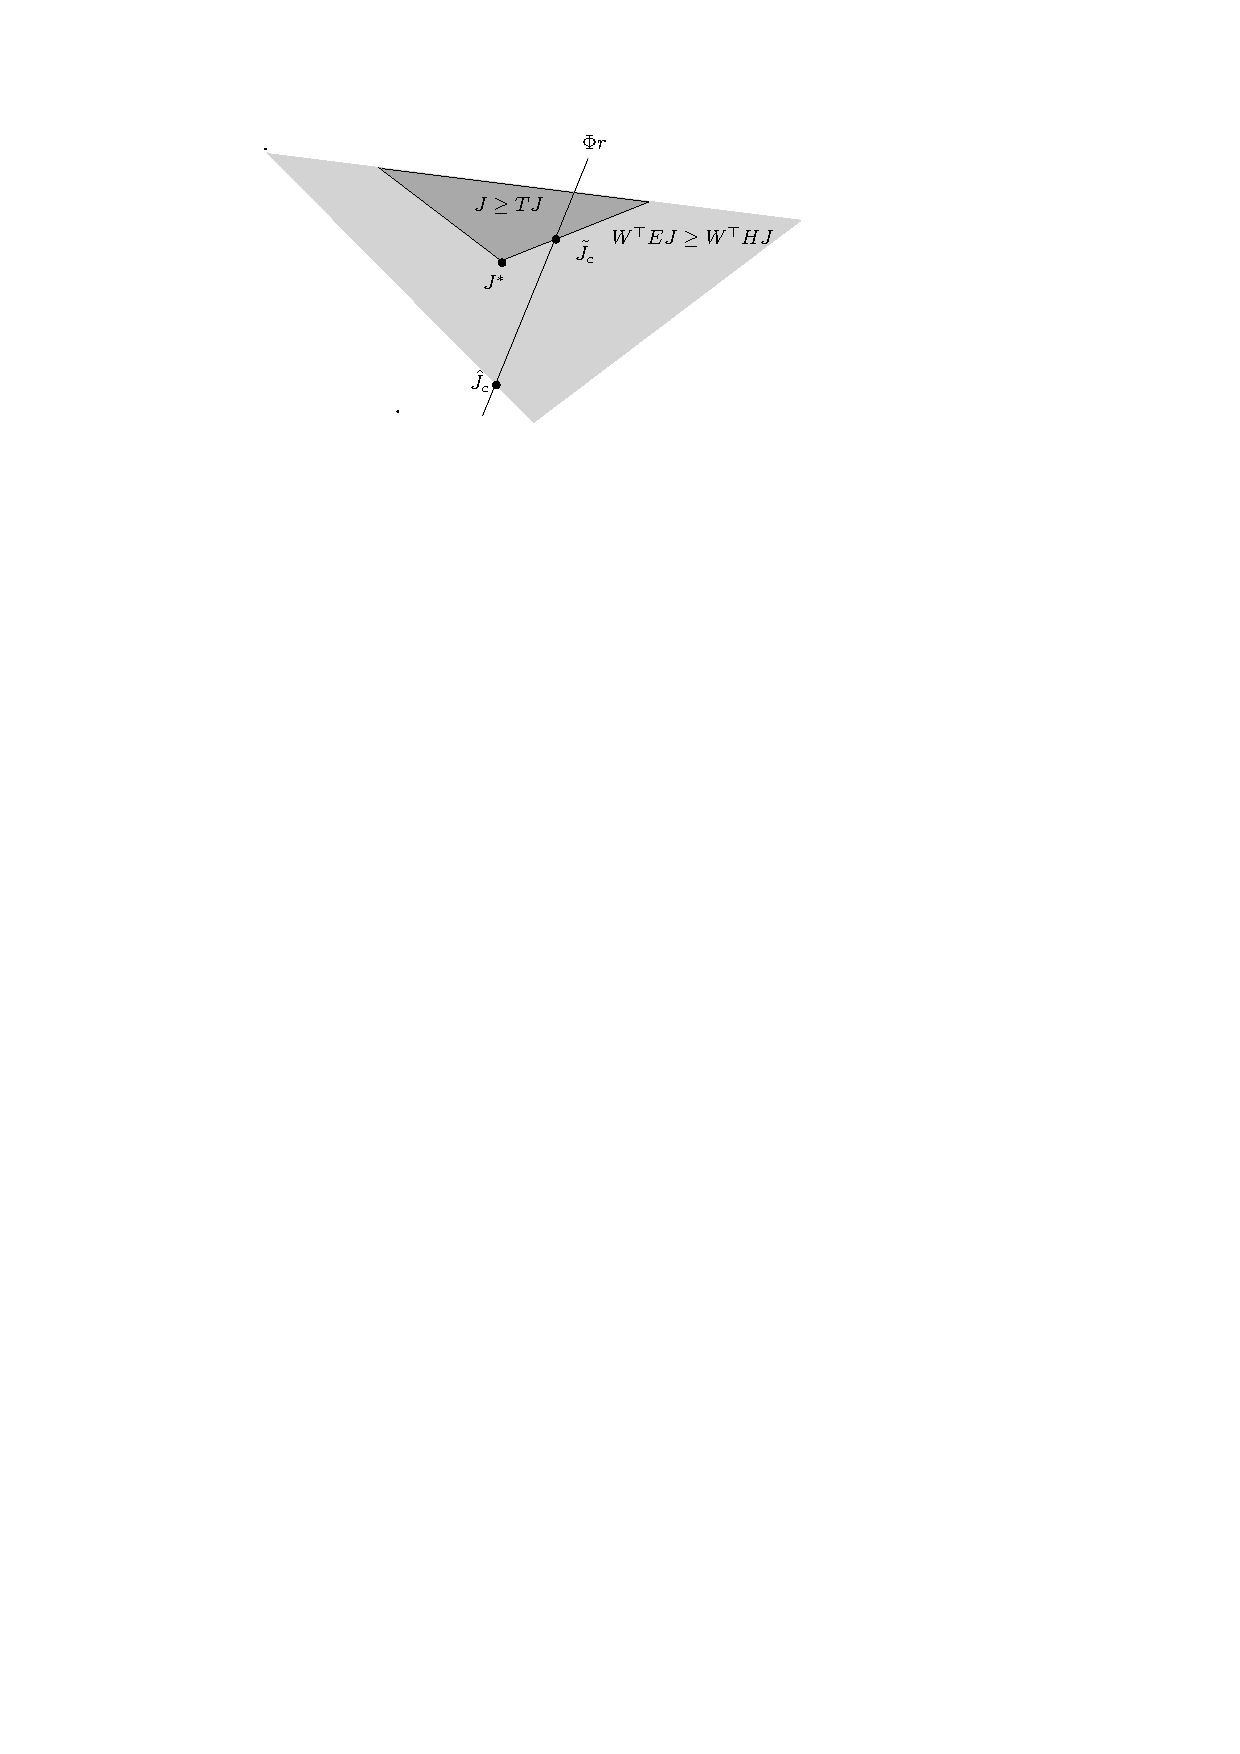
\includegraphics[scale=0.7]{cartoon_grlp.pdf}
\caption{
%\normalsize
The outer lightly shaded region corresponds to GRLP constraints and the inner dark shaded region corresponds to the original constraints. The main contribution of the paper is to bound $\norm{J^*-\hat{J}_c}$.}
\label{cartoon}
\end{figure}
\Cref{cartoon} shows the solutions to the LP, ALP and GRLP respectively. The error in ALP solution has already been studied in \cite{ALP}. Our objective is to study the extra source of error due to constraint approximation.
\fi

%\subsection{Error Bounds}
%%%%%%%%%%%%%%%%%%%%%%%%%%%%%%%%%%%%%%%%
\begin{theorem}[Error Bound for LRALP]
\label{cmt2}
Assume that $c\in \Re_+^S$ is such that $1^\top c = 1$ and that $W \in \Re_+^{SA\times m}$ is nonnegative valued.
Let $\psi\in \Re_+^S$ be in the column span of $\Phi$ and assume that the $\alpha$-discounted stability coefficient of $\psi$ is $\beta_\psi<1$. 
Let $\eps = \inf_{r\in \Re^k}\norm{J^*-\Phi r}_{\infty,\psi}$ 
be the error of approximation $J^*$ using the basis functions in $\Phi$.
Then,
\begin{align*}
\norm{J^*-\hj}_{1,c} \leq 
 \frac{2 c^\top \psi}{1-\beta_\psi} \left(
	2.5 \eps
     +\norm{\Jalpo-\Jlro}_{\infty,\psi}\right)\,.
\end{align*}
%%%%%%%%%%%%%%%%%%%%%%%%%%%%%%%%%%%%%%%%
\if0
\item The control error is bound as\\
$\norm{J^* - J_{\hu}}_{1,c}
\leq 2\left(\frac{1}{(1-\alpha)^2}\right)\, \big( 2~\us{\min}{r\in \Re^k} \norm{J^*-\Phi r}_{\infty}
+\norm{\Gamma J^*-\hg J^*}_{\infty}+\norm{\hj-\hg\hj}_{\infty}\big)$.
\end{enumerate}
\fi
\end{theorem}
%%%%%%%%%%%%%%%%%%%%%%%%%%%%%%%%%%%%%%%%
Note that the result implicitly assumes that $\hj$ exists, because if $\hj$ does not exist then $\Jlro$ is necessarily unbounded, making the last error term infinite. To ensure that $\psi$ is in the span of $\Phi$, after choosing $\psi$, one can add $\psi$ as one of the basis functions. Alternatively, the bound can also be interpreted to hold for any $\psi$ in the span of $\Phi$ with $\beta_\psi<1$.

As noted earlier, \citet{ALP} prove a similar error bound for $\Jalp$, the solution of the ALP.
In particular, their Theorem 3 states that  under identical assumptions as in our result,
$\norm{J^* - \Jalp}_{1,c} \le \frac{2 c^\top \psi \epsilon}{1-\beta_\psi}$ for $\epsilon$ defined as above
 (the result we cited previously is a simplified form of this bound).
The larger coefficient of $\epsilon$ is probably an artifact of our analysis. 
Note that when $W$ does not reduce the constraints, 
our bound is only a constant factor larger than this previous result.
The extra term $\norm{\Jalpo-\Jlro}_{\infty,\psi}$ can be seen as the price paid for relaxing the constraints.

From linear programming theory, it follows that primal boundedness is equivalent to dual feasibility. 
Since the dual of $\min\{c^\top x\,:\, Ax \ge b \}$ is 
$\max\{ y^\top b\,:\, y \ge 0, c = A^\top y\}$, we get
that a necessary and sufficient condition for $\Jlro$ 
to be finite-valued is that for any $s\in \S$, $\phi(s)$ lies in the conic span, 
$\{ U \lambda\,:\, \lambda\in \Re_+^{SA}\}$, of (the columns) of $U = \Phi^\top E^\top W$.
%(Note that the boundedness of LRALP only requires that $\Phi^\top c$ lies in the conic span of $U$.)
When $W$ is such that its constituents $W_1,\dots,W_A$ are all identical, 
the conic span of $U$ is equal to the conic span of $\Phi^\top W_1$. 
It is particularly instructive 
to consider the case when the common matrix $W_a = (w_{1,a},\dots,w_{m,a})$ ``selects'' the $m$ states,
i.e., when $\{w_{1,a},\dots,w_{m,a}\}= \{ e_{s}\,:\, s\in \S_0 \}$ for some $\S_0\subset \S$, $|\S_0|\le m$,
where $e_s\in \{0,1\}^\S$ are the $s\in \S$ vectors in the standard Euclidean basis.
In this case, the condition that $\phi(s)$ lies in the conic span of $U$ 
is equivalent to that $\phi(s)$ lies in the conic span of $\phi(\S_0) \doteq \{\phi(s')\,:\, s'\in \S_0\}$. 
Thus, to ensure boundedness of $\Jlro$, 
the chosen states should be selected to ``conicly cover'' all the vectors in $\phi(\S)\subset \Re^k$.%
\footnote{The same implies that, under the same condition on $W$, boundedness of the LRALP 
holds if and only if $\sum_s c(s) \phi(s)$ is in the conic span of $\phi(\S_0)$. Note that this is easy to fulfill
if the support of $c$ has a small cardinality by add all states in the support of $c$ to $\S_0$.
}

The next theorem shows that magnitudes of the coefficients used in the conic cover control the size of 
$\norm{\Jalpo-\Jlro}_{\infty,\psi}$. 
For the theorem we let $\Lambda\in \Re_+^{\S\times \S_0}$ be the matrix of conic coefficients: 
For any $s\in \S$, $\phi(s) = \sum_{s'\in \S_0} \Lambda(s,s') \phi(s')$. After the theorem we give constructions 
for creating conic covers.
\begin{theorem}
\label{conetheorm}
Assume that $W_1 = \dots = W_A$, $\{w_{1,a},\dots,w_{m,a}\} = \{ e_s\,:\, s\in \S_0 \}$ 
and that $\phi(\S)$ lies in the conic span of $\phi(\S_0)$ with conic coefficients given by $\Lambda$.
Let $\epsilon = \inf_{r}\norm{ J^* -  \Phi r }_{\infty,\psi}$.
Then, 
\begin{align*}
\norm{\Jalpo-\Jlro}_{\infty,\psi}
\le 
\norm{\Jalpo-J^*}_{\infty,\psi} + (1+ \norm{\Lambda \psi}_{\psi,\infty}) \epsilon\,.
\end{align*}
\end{theorem}
\begin{proof}
Let $r^*$ be such that $\norm{J^* - \Phi r^*}_{\infty,\psi} = \epsilon$ (this exists by continuity) and let 
$\delta = J^* - \Phi r^*$.
Pick any $s\in \S$ and let $r_s = \argmin\{ r^\top \phi(s) \,:\, W^\top E \Phi r \ge W^\top E J^*,\, r\in \Re^k \}$ 
so that $\Jlro(s) = r_s^\top \phi(s)$.
Note that by assumption, for any $s'\in \S_0$, $\Jlro(s') = r_s^\top \phi(s') \ge J^*(s')$.
Now, notice that by definition, $\Jlro \le \Jalpo$ (the LP defining $\Jlro$ is the relaxation of the LP defining $\Jalpo$).
Hence,
$%\begin{align*}
0\le \Jalpo(s) - \Jlro(s) = \Jalpo(s) - J^*(s) + J^*(s) - \Jlro(s)
$% \end{align*}
and $\Jlro(s) = r_s^\top \phi(s) = r_s^\top \sum_{s'\in \S_0} \Lambda(s,s') \phi(s') = \sum_{s'\in \S_0} \Lambda(s,s') \Jlro(s')
\ge \sum_{s'\in \S_0} \Lambda(s,s') J^*(s')$.
Combining this with the previous inequality we get
$%\begin{align*}
0\le
%&\le 
 \frac{\Jalpo(s) - \Jlro(s)}{\psi(s)}\\
 \le
%&\le
\frac{\Jalpo(s)-J^*(s)}{\psi(s)} + \frac{J^*(s) - \sum_{s'\in \S_0} \Lambda(s,s') J^*(s')}{\psi(s)}
%\,.
$. % \end{align*}
Plugging in $J^*(s) = \phi(s)^\top r^*+\delta(s)$, using again that $\phi(s) = \sum_{s'\in \S_0} \Lambda(s,s') \phi(s')$,
and also using the triangle inequality after taking absolute values, we get
\begin{align*}
\MoveEqLeft \frac{|J^*(s) - \sum_{s'\in \S_0} \Lambda(s,s') J^*(s')|}{\psi(s)} \\
& \le
  \frac{|\delta(s)|}{\psi(s)} + \frac{\sum_{s'\in \S_0} \Lambda(s,s') |\delta(s')|}{\psi(s)} \\
%& \le
%  \frac{|\delta(s)|}{\psi(s)} + \frac{1}{\psi(s)} \, \sum_{s'\in \S_0} \Lambda(s,s') \psi(s') \frac{|\delta(s')|}{\psi(s')} \\
& \le
  \frac{|\delta(s)|}{\psi(s)} + \norm{\delta}_{\infty,\psi} \frac{\sum_{s'\in \S_0} \Lambda(s,s') \psi(s')}{\psi(s)} \, .
\end{align*}
Combining this with the previous display and noting that $\norm{\delta}_{\infty,\psi} = \epsilon$ finishes the proof.
\if0
Putting things together, we get 
\begin{align*}
\norm{\Jalpo - \Jlro}_{\infty,\psi}
\le
\norm{\Jalpo(s)-J^*(s)}_{\infty,\psi}
+ 
\norm{\delta}_{\infty,\psi} (1+ \norm{\Lambda \psi}_{\infty,\psi})\,,
\end{align*}
finishing the proof.
\fi
\end{proof}

Given $\phi:\S \to \Re^k$, what is the minimum cardinality set $\S_0$ that 
conicly covers $\phi(\S)$ and how to find such a set? Further, how to keep the magnitude of $\norm{\Lambda \psi}_{\infty,\psi}$ small? To control this latter quantity it seems essential to make sure $\S_0$ contains states with high $\psi$-values. 
However, if one is content with a bound that depends on $\norm{\psi}_{\infty}$, one can bound 
$\norm{\Lambda \psi}_{\infty,\psi}$ by $\norm{\psi}_{\infty} \zeta$ where $\zeta = \max_s \sum_{s'\in \S_0} \Lambda(s,s')$,
hence, the second term in the previous bound will be bounded by $(1+\norm{\psi}_{\infty} \zeta) \eps$.

Let us now return to the problem of finding conic covers. 
We will proceed by considering some illustrative examples. 
As a start, consider the case when the basis functions are binary valued.
In this case, it is sufficient and necessary to choose one state for each binary vector 
that appears in $\phi(\S)\subset \{0,1\}^k$.
This gives that $m_0 \doteq |\S_0|\le 2^k$ representative states will be sufficient \emph{regardless of the cardinality of $\S$}.
Further, in this case $\zeta = 1$.
For moderate to large $k$ (e.g., $k\gg 20$), it will quickly become infeasible to keep $2^k$ constraints.
In this case we may need to restrict what features are considered to guarantee the conic cover condition.
Letting $A_i = \{s\in \S\,:\, \phi_i(s)=1 \}$, if for a many pairs $i\ne j$, $A_i$ and $A_j$ do not overlap 
then $N = |\phi(\S)|$ can be much smaller than $2^k$. 
For example, in the commonly used state aggregation procedures 
$A_i \cap A_j = \emptyset$ for any $i\ne j$, giving $N=k$. 
%In this case $N=k$: It suffices to choose one representative state from each of the $A_i$ sets and add them to the constraints. 
In the more interesting case of 
hierarchical aggregation (when the sets $\{A_i\}$ form a nested hierarchical partitioning of $\S$), 
we have $m_0 \le D \cdot k$ where $D$ is the depth of the hierarchy.

Another favourable example is the case of separable bases.
In this case, the states are assumed to be factored 
and the basis functions depend only on a few factors.
Let us consider a simple illustration.
By abusing notation (redefining $\S$), let $\S = \S_1 \times \S_2$, 
let there be $k=2$ basis functions and assume that $\phi_i(s) = h_i(s)$ for some $h_i:\S_i \to \Re$, $i=1,2$.
Assume further that $0\in h_i(\S_i)$ for both $i$ and specifically let $s_{i0}$ be such that $h_i(s_{i0})=0$.
In this case it is not hard to verify that if $\S_{i0}$ is such that $h_i(\S_i)$ is in the conic span of $h_i(\S_{i0})$ then
$\phi(\S)$ is also in the conic span of $\S_0 \doteq \S_1 \times \{ s_{20} \} \cup \{ s_{10} \} \times \S_2$.
The point is that $|\S_0| \le |\S_1| + |\S_2|$, which is a tolerable increase of growth.
This example is not hard to generalize to more general, ANOVA-like basis expansions. The moral
is that as long as their limited order of interaction (which is usually necessary for information theoretic reasons as well),
the number of constraints may grow moderately with the number of factors (dimensionality) of the state space.

In some cases, finding a conic cover with a small cardinality is not possible. 
This can already happen in simple examples such as when $\S = \{1,\dots,S\}$ (as before) and
$\phi( s ) = (1,s,s^2)^\top$. In this case, the only choice is $\S_0 = \S$. 
In examples similar to this one one possibility is to quantize the range of $\phi$, which may  loose
little on approximation quality, while it creates the opportunity 
to construct a small cardinality conic cover.

Note that the bound of \cite{CS} and our main result can be seen as largely complementary. 
Recall that \citeauthor{CS} consider adding an extra constraint $r\in \N$, while they propose to select all $A$ constraints
from the ALP corresponding to $m$ states chosen at random from some distribution $\mu$. 
Then, with high probability,
they show that, provided that $\ralp \in \N$,
 the extra price paid for relaxing the constraints of the ALP is $O( \rho \epsilon_{\N} k/m)$,
 where $\rho = \max_{s} \frac{\mu^*(s)}{\mu(s)}$, $\mu^* = (1-\alpha)c^\top (I-\alpha P_{u^*})^{-1}$, $u^*$ is an optimal policy,
and $\epsilon_{\N} = \sup_{r\in \N} \norm{J^*-\Phi r}_{\infty,\psi}$.%
\footnote{The paper presents the results for $\mu = \mu^*$ giving $\rho=1$, but the analysis easily extends to the general case.}
The bound is nontrivial when $m\ge \rho \epsilon_{\N} k$.
In general, it may be hard to control $\rho$, or even $\epsilon_{\N}$ while ensuring that $\ralp \in \N$.



\if0
\textbf{On Prediction Error:} The first factor in the right hand side of the prediction error in \Cref{cmt2} is related to the best possible approximation that can be achieved with the chosen feature matrix $\Phi$. This term is an carry over of the upper bound in ALP formulation as shown in \Cref{alpvanilla}. The second factor in the right hand side of the prediction error is related to constraint approximation and is completely defined in terms of $\Phi$, $W$ and $T$, and does not require knowledge of stationary distribution of the optimal policy.\par
\textbf{On Control Error:} The first two terms are quite similar to those in the bound for prediction error. The third term occurs due to the fact that $\Phi \geq T\Phi r$ that holds in the case of ALP does not hold in the case of GRLP.\par
\begin{comment}
\begin{theorem}[Control Error Bound in $\norm{\cdot}_{\infty}$]
\label{polthe}
Let $\hu$ be the greedy policy with respect to the solution $\hj$ of GRLP and $J_{\hu}$ be its value function.
% Let $r^*$ be as in Theorem~\ref{mt2mn}, then
Then,
\begin{align}\label{polthebnd}
\norm{J^* - J_{\hu}}_{1,c}
&\leq 2\left(\frac{c^\top \psi}{(1-\beta_{\psi})^2}\right)\, \big( 2\norm{J^*-\Phi r^*}_{\infty}
\nn\\&
+norm{\Gamma J^*-\hg J^*}_{\infty}+\norm{\hj-\hg\hj}_{\infty}\big).
\end{align}
\end{theorem}
\end{comment}
\begin{corollary}[Constraint Sampling]\label{st}
$W\in \{0,1\}^{nd\times m}$Let $s\in S$ be a state whose constraint is selected by $W$ (i.e., for some $i$ and all $(s',a)\in S\times A$,
$W_{s'a,i}=\delta_{s=s'}$.
Then
\begin{align*}%\label{sampexp}
|\Gamma J^*(s)-\hg J^*(s)|<|\Gamma J^*(s)-J^*(s)|.
\end{align*}
\end{corollary}
It is important to note that \Cref{rlpt} holds only in high probability and is valid only under idealized assumption of knowing the optimal policy $u^*$, while \Cref{cmt2} does not have these limitations.
In addition, the error $|\Gamma J^*(s) -\hg J^*(s)|$ (in \Cref{st} ) due to constraint approximation is less than the original projection error $|\Gamma J^*(s)-J^*(s)|$ due to function approximation. This means that for RLP to perform well it is important to retain the constraints corresponding to those states for which the linear function approximation via $\Phi$ is known to perform well.
\fi

